\documentclass[11pt]{article}
\def\AtlasMain{1}
\usepackage[margin=0.85in]{geometry}
\usepackage{amsmath,amssymb,graphicx,booktabs,array,float}
\usepackage{tikz}
\usetikzlibrary{arrows.meta,positioning}
\usepackage{xcolor,hyperref,fancyhdr}
\definecolor{ink}{HTML}{163447}
\definecolor{teal}{HTML}{167E79}
\hypersetup{colorlinks=true,urlcolor=teal,linkcolor=teal,citecolor=teal,
pdftitle={From Molecular Trajectories to Composable Paths},
pdfauthor={Joseph Campagna, PSM}}
\usepackage[T1]{fontenc}
\usepackage{lmodern}
\setlength{\parindent}{0pt}
\setlength{\parskip}{6pt}
\setlength{\emergencystretch}{2em}
\renewcommand{\arraystretch}{1.15}
\pagestyle{fancy}\fancyhf{}
\fancyhead[L]{\small\textcolor{ink}{MOLECULAR ATLAS / EXPLORATORY NOTE}}
\fancyhead[R]{\small October 2026}
\fancyfoot[L]{\small Computational visualization; not peer reviewed}
\fancyfoot[R]{\thepage}
\setlength{\headheight}{15pt}
\newcommand{\Cat}{\mathcal C}
\newcommand{\N}{\mathrm N}
\newcommand{\R}{\mathbb R}
\newcommand{\T}{\mathbb T}
\begin{document}
{\color{ink}\LARGE\bfseries From Molecular Trajectories\\to Composable Paths\par}
\vspace{4pt}
{\large Alanine dipeptide and the chignolin variant CLN025\par}
\textbf{Joseph Campagna, PSM}\hfill October 2026

\textbf{Abstract.}
Can molecular geometry make the composition of dynamical behavior visible?
We construct an interactive atlas from 750,000 public molecular dynamics (MD)
frames of alanine dipeptide and 1,868,861 frames from the complete public
deposit of the ten-residue chignolin variant CLN025. The revised landscape
uses supported structural mobility in nm, recorded molecular relief, and
an explicitly root-balanced descriptive estimator for CLN025. Two distinct
categorical constructions remain distinguished:
an overlap face-poset nerve and a free path-category nerve derived from observed
basin passages. Legacy translucent morphing skins are retained as illustrative
baselines; the measured viewer steps through recorded conformers without
synthetic molecular interpolation. Train-only grouped prediction, kinetic
diagnostics, chemical mapping and higher-simplex audits constrain interpretation.
This construction remains an exploratory vocabulary for discussing composition.
It is not a claim of recovered configuration-space topology, a validated
Markov model, or a completed theory of compositional protein dynamics.
The prototype motivates an experimentally testable route from trajectory
composition toward composition of open dynamical subsystems.

\begin{figure}[H]
\centering
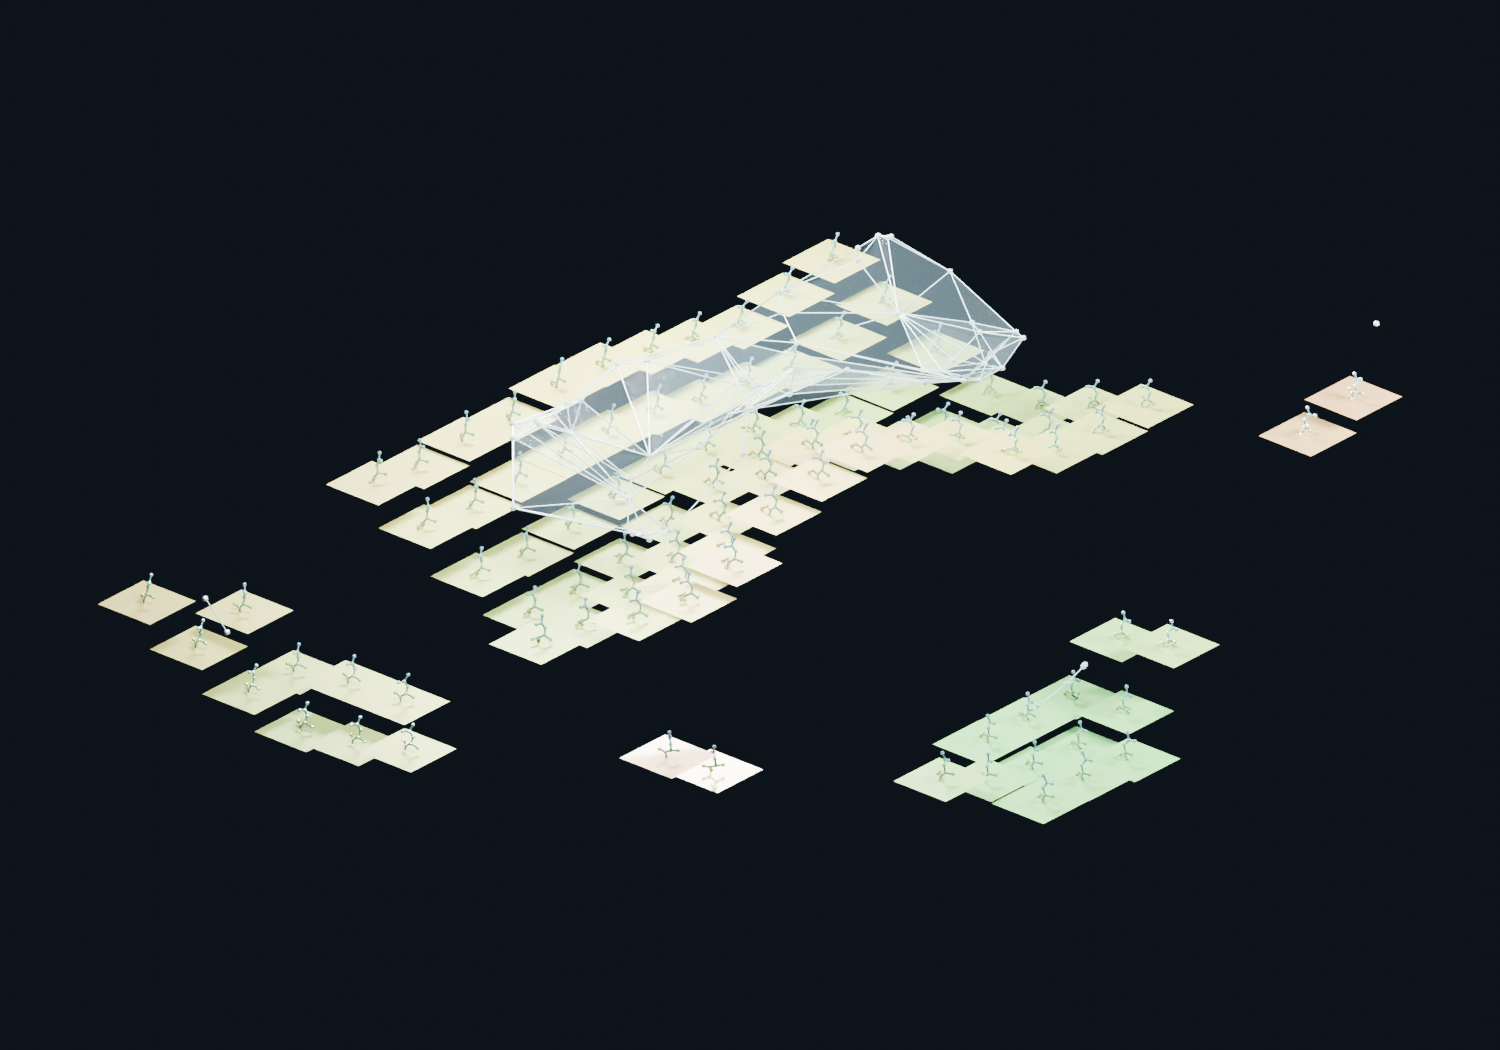
\includegraphics[width=.78\linewidth]{figures/alanine-measured-landscape.png}
\caption{\textbf{Alanine: measured mobility with recorded molecular relief.}
Blender 4.0/Cycles rendering. Tile height encodes the conditional RMS change
in internal pair distances at a 100 ps lag; absent tiles have insufficient
support. Recorded molecules are rigidly aligned and separately magnified.
The lifted nerve shows inclusions and triangular chains; its display offset
is not a physical coordinate. Gloss and lighting are optical aids, not additional
observables. Numerical scales and uncertainty are supplied in Figure 9.}
\end{figure}

\textbf{Explore the artifact.}
\href{https://joecampdb.github.io/pronerv_MTNerv/}{Interactive molecular atlas}
and \href{https://github.com/joecampdb/pronerv_MTNerv}{public source repository}.
The public viewer is the historical illustrative baseline. The local revised
\texttt{measured.html} supports recorded frames, supported mobility, uncertainty,
periodic viewing and independent nerve overlays. Its deployment and a revised
full-paper PDF are separate release steps. All figures are generated from
the numerical geometry; they are not AI-generated illustrations.

\newpage
\section*{Molecular systems and cartoon conventions}
The two cases share a categorical construction, but differ in molecular
resolution and chart coordinates. Alanine dipeptide is represented by ten
heavy atoms. CLN025 is represented by ten C$\alpha$ sites, one per residue:
the equal site counts do not imply equal molecular complexity.

\begin{figure}[H]\centering
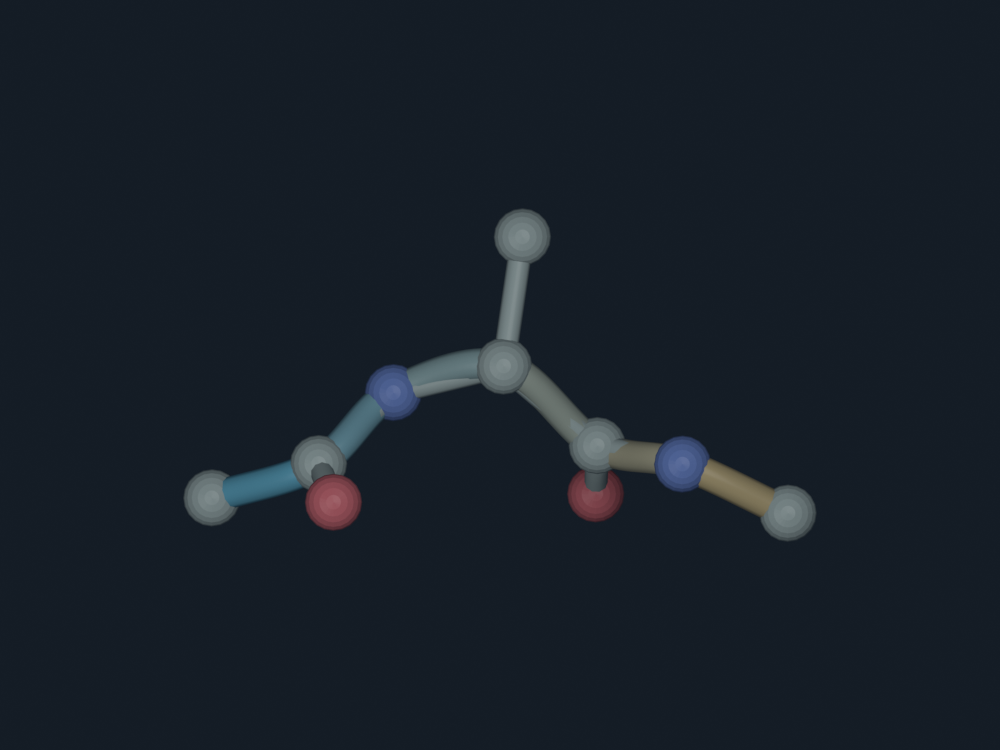
\includegraphics[width=.43\linewidth]{figures/alanine-cartoon.png}
\caption{\textbf{Alanine dipeptide: a backbone cartoon with atomic context.}
The blue-to-gold tube traces the capped backbone from one end to the other;
heavy atoms and bonds retain chemical context (oxygen red, nitrogen blue).
Coordinates come from the recorded representative of overlap object $U_0$.
A helix/sheet ribbon would not be meaningful for this short benchmark.}
\end{figure}
\begin{figure}[H]\centering
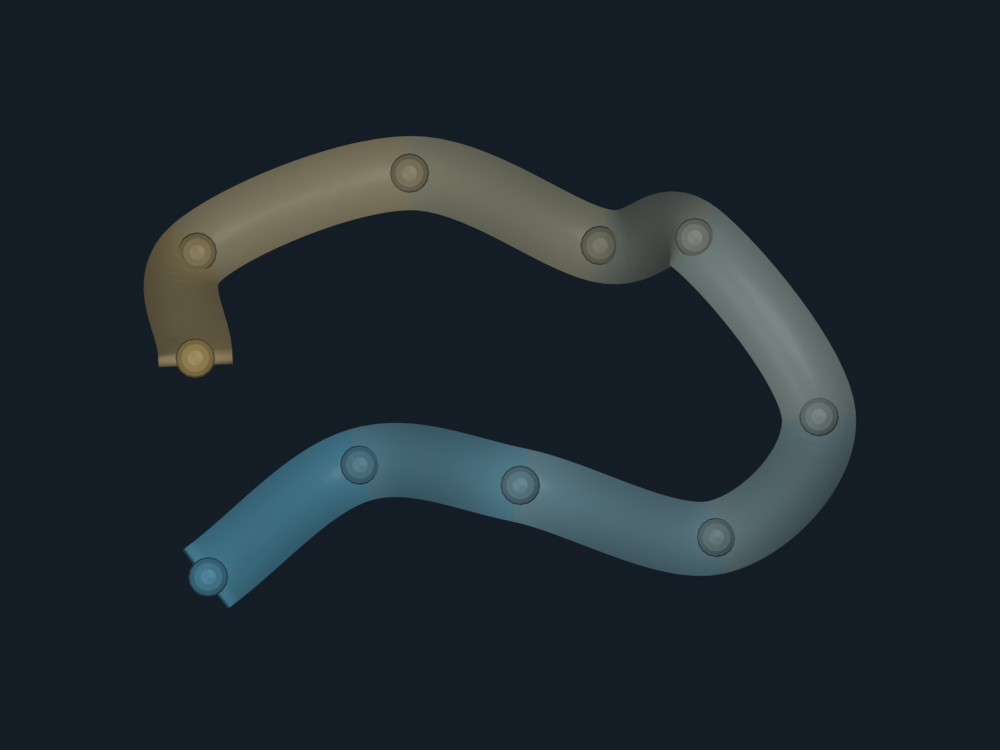
\includegraphics[width=.48\linewidth]{figures/chignolin-compact-cartoon.png}\hfill
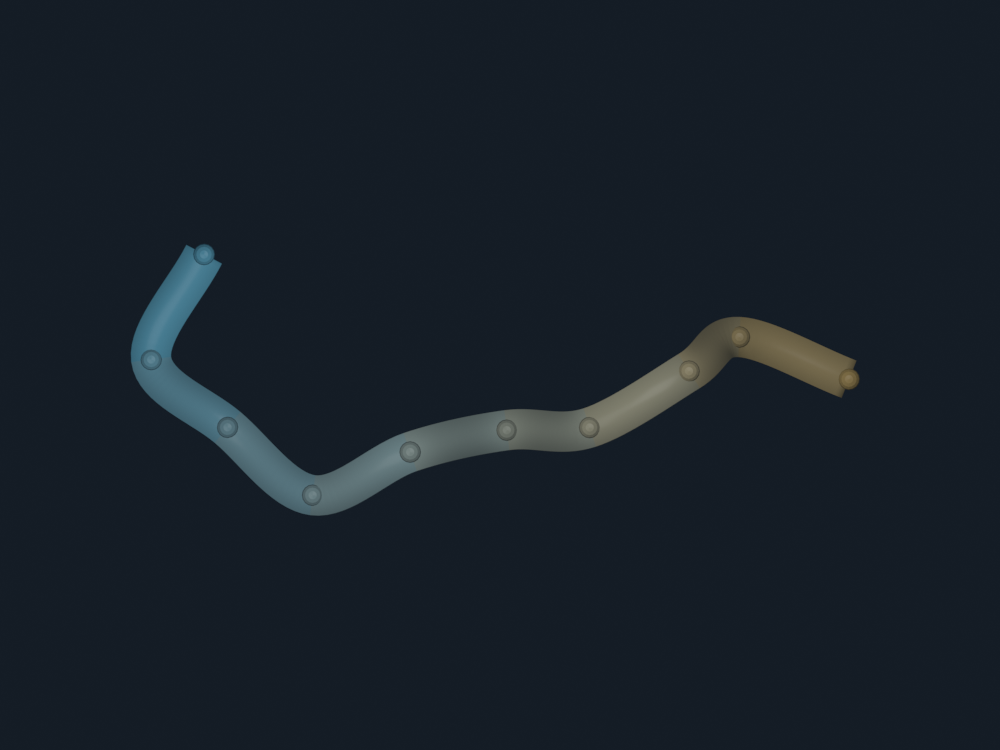
\includegraphics[width=.48\linewidth]{figures/chignolin-extended-cartoon.png}
\caption{\textbf{Chignolin CLN025: compact and extended C$\alpha$ cartoons.}
Sequence YYDPETGTWY. Actual frames nearest the 5th and 95th percentiles of
C$\alpha$ radius of gyration are shown. Ribbons interpolate the recorded
C$\alpha$ sites; blue-to-gold indicates N-to-C order. These are geometric
backbone cartoons, not DSSP secondary-structure assignments or assertions of
native and unfolded states. Each panel has its own fitted camera scale.}
\end{figure}
The cartoons and landscape figures were rendered in Blender from exported
MD coordinates. Smooth ribbons and tubes are illustrative interpolation between
sites. The CLN025 mutation and capping conventions are inherited from the
deposited simulation topology; the example is not mislabeled as wild-type
chignolin. The viewer provides corresponding backbone-trace insets, recorded
representatives, and animated route conformations.

\newpage
\section*{1. Two nerves, two meanings of composition}
For alanine, let $q_t=(\phi_t,\psi_t)\in\T^2$ describe the backbone angles, and let
$X_t\in\R^{10\times3}$ contain the aligned heavy-atom coordinates.
Alanine dipeptide is a capped amino-acid benchmark, not a folded protein.
Its small conformational chart makes the distinctions below inspectable.

\textbf{Overlap category.}
Take 18 balls of radius $55^\circ$ in the periodic angular metric. The finite
sample $W$ contains all 750,000 available frames and witnesses membership:
\[
 K_W=\{\sigma\ne\varnothing:\exists q\in W,\ q\in\bigcap_{i\in\sigma}U_i\}.
\]
We store maximal simplices of the full witnessed complex, and draw the
face-poset category of its 2-skeleton,
$\Cat_{\cap}=P(K_W^{(2)})$. Objects are simplices; arrows are inclusions
of index sets, not reverse inclusions of intersection regions.
Its nerve has 78 objects, 212 strict inclusions, and 138 nondegenerate
2-simplices. The realization is a barycentric subdivision:
\[
 |\N P(K_W^{(2)})|\cong |K_W^{(2)}|.
\]
This categorical statement does not establish equivalence with the protein's
configuration space. Good-cover hypotheses and sampling guarantees are
separate issues \cite{may,bauer}. The measured viewer includes a torus view;
flat-view seam-crossing geometry is omitted without deleting categorical data.

\textbf{Dynamic path category.}
Let $G$ have four basin objects and ten directed generators, one for each
observed route type (CLN025 has twelve generators). Set $\Cat_{\rm path}=\mathrm{Free}(G)$.
Morphisms are finite composable words; identities are empty words.
For any category,
\[
 \N(\Cat)_n=\operatorname{Fun}([n],\Cat)
 =\{x_0\xrightarrow{f_1}\cdots\xrightarrow{f_n}x_n\}.
\]
Inner face maps compose adjacent arrows; degeneracies insert identities.
For a 2-simplex $(f,g)$, $d_0(f,g)=g$, $d_1(f,g)=g\circ f$,
and $d_2(f,g)=f$. Thus the long edge is a composite, not a missing
observation to be filled in.

\begin{figure}[H]\centering
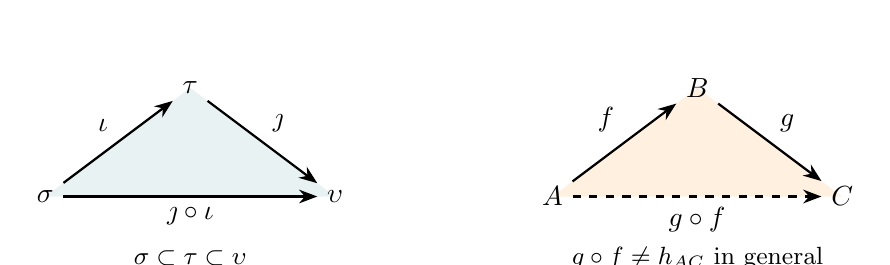
\begin{tikzpicture}[>=Stealth,scale=.92]
\fill[teal!10] (0,0)--(2,1.5)--(4,0)--cycle;
\node (s) at (0,0) {$\sigma$};\node (t) at (2,1.5) {$\tau$};\node (u) at (4,0) {$\upsilon$};
\draw[->,thick] (s)--node[above left] {$\iota$}(t);
\draw[->,thick] (t)--node[above right] {$\jmath$}(u);
\draw[->,thick] (s)--node[below] {$\jmath\circ\iota$}(u);
\node at (2,-.85) {\small $\sigma\subset\tau\subset\upsilon$};
\fill[orange!12] (7,0)--(9,1.5)--(11,0)--cycle;
\node (a) at (7,0) {$A$};\node (b) at (9,1.5) {$B$};\node (c) at (11,0) {$C$};
\draw[->,thick] (a)--node[above left] {$f$}(b);
\draw[->,thick] (b)--node[above right] {$g$}(c);
\draw[->,thick,dashed] (a)--node[below] {$g\circ f$}(c);
\node at (9,-.85) {\small $g\circ f\ne h_{AC}$ in general};
\end{tikzpicture}
\caption{\textbf{The two displayed simplicial meanings.}
Left: composition of inclusions. Right: formal composition of route generators.
An independently observed $A\to C$ generator $h_{AC}$ remains a different arrow.
The displayed 25 alanine pairs (36 for CLN025) are only a finite view of
the infinite path-category nerve. Return paths are not identities.}
\end{figure}
The two categories coexist as overlays. No functor identifying them has been
constructed. Likewise, a composable pair need not occur consecutively in the
recorded MD trajectory.

\newpage
\section*{Geometric atlas of the overlap nerve}
The following plates show the complete exported overlap-nerve 2-skeletons,
with identical connectivity in oblique and overhead views.
Each vertex represents an object of the face poset: a witnessed index set
$\sigma\in K_W^{(2)}$. Circles, squares and triangles distinguish
$|\sigma|=1,2,3$; all three marker types are vertices of the categorical nerve.
An edge represents a strict inclusion $\sigma\subset\tau$.
A filled triangular face represents a composable chain
$\sigma\subset\tau\subset\upsilon$ and includes the composite edge
$\sigma\subset\upsilon$. Line direction is suppressed for visual clarity;
inclusion always points from the smaller to the larger index set.

\begin{figure}[H]\centering
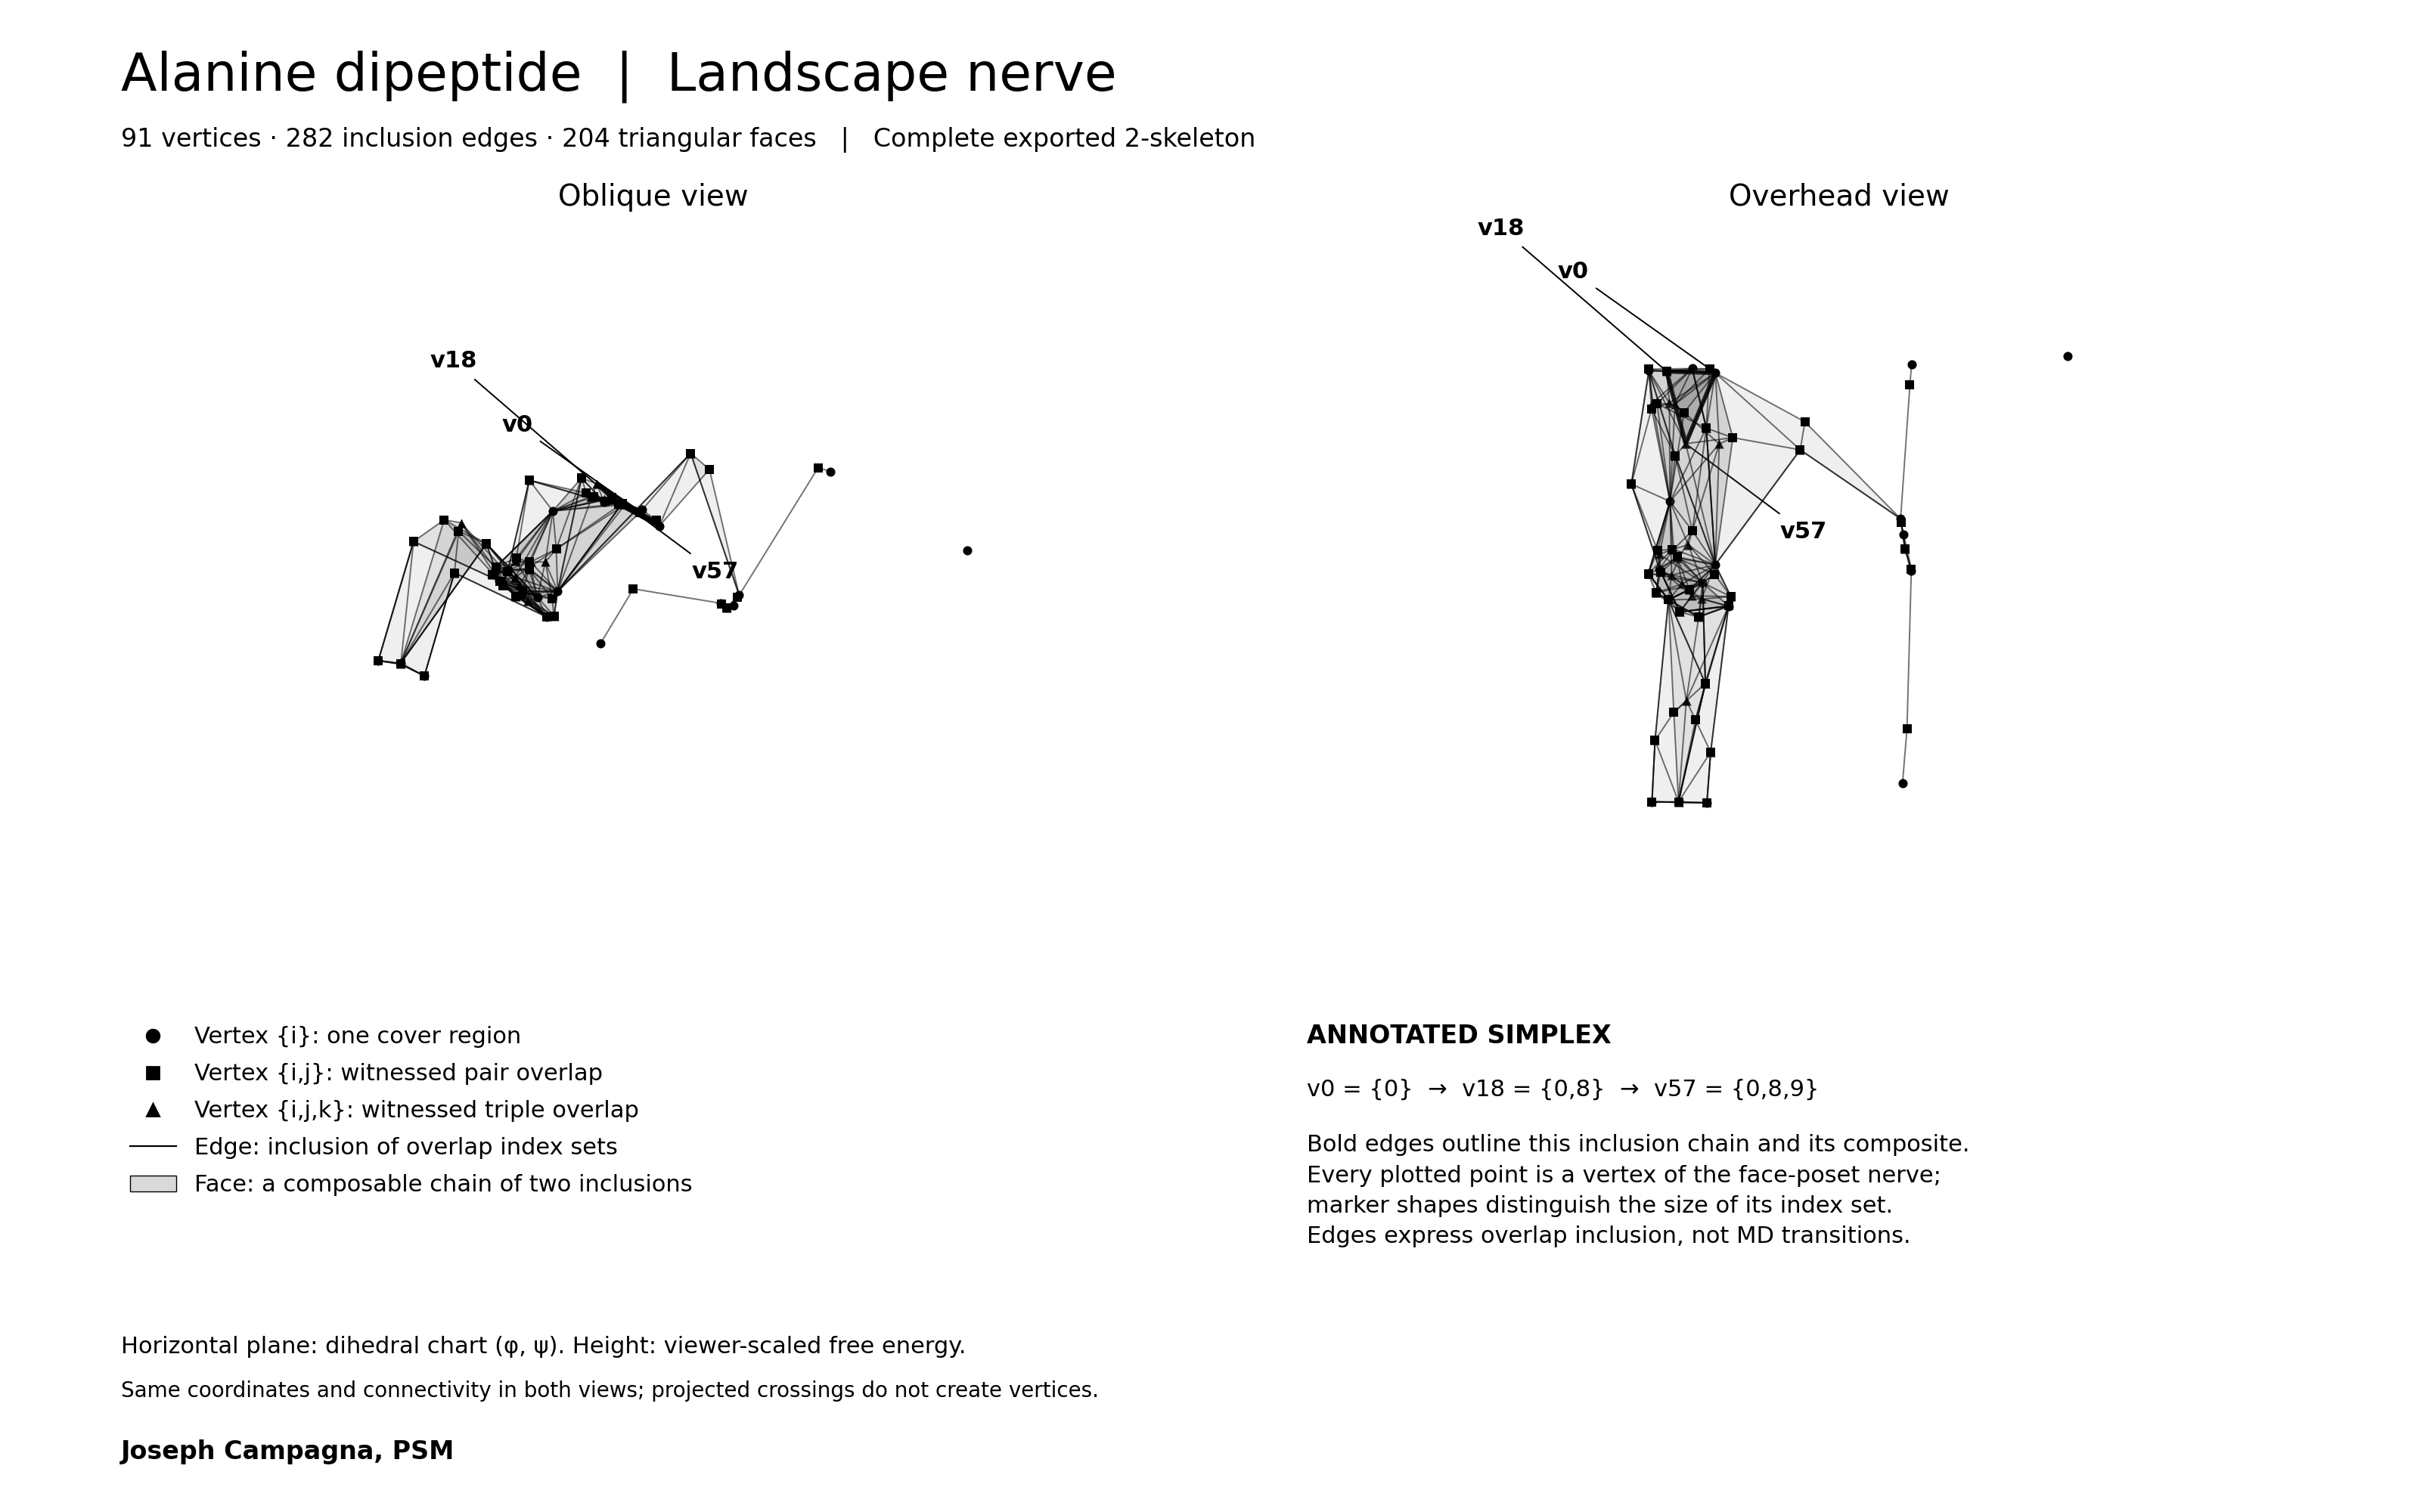
\includegraphics[width=\linewidth]{figures/alanine-nerve-annotated-both.png}
\caption{\textbf{Alanine: the full exported overlap nerve in two views.}
All 91 vertices, 282 strict inclusion edges and 204 triangular faces are
displayed. The labeled example is
$v_0=\{0\}\subset v_{18}=\{0,8\}\subset v_{57}=\{0,8,9\}$.
Vertex IDs are zero-based indices in the exported node array.
Horizontal coordinates follow the viewer's cut $(\phi,\psi)$ chart;
height follows its scaled empirical free-energy coordinate.
The shape is an embedding of the exported combinatorics, not a reconstructed
physical molecular surface.}
\end{figure}
The vertex positions are recorded representatives of the corresponding overlaps,
not necessarily geometric barycenters. Thus the displayed linear triangles
can cross or overlap in projection. These crossings do not create new vertices
or alter the abstract nerve. The categorical realization statement above
concerns the abstract complex, not an injective embedding in this chart.

\newpage
\section*{Geometric atlas of the CLN025 overlap nerve}
\begin{figure}[H]\centering
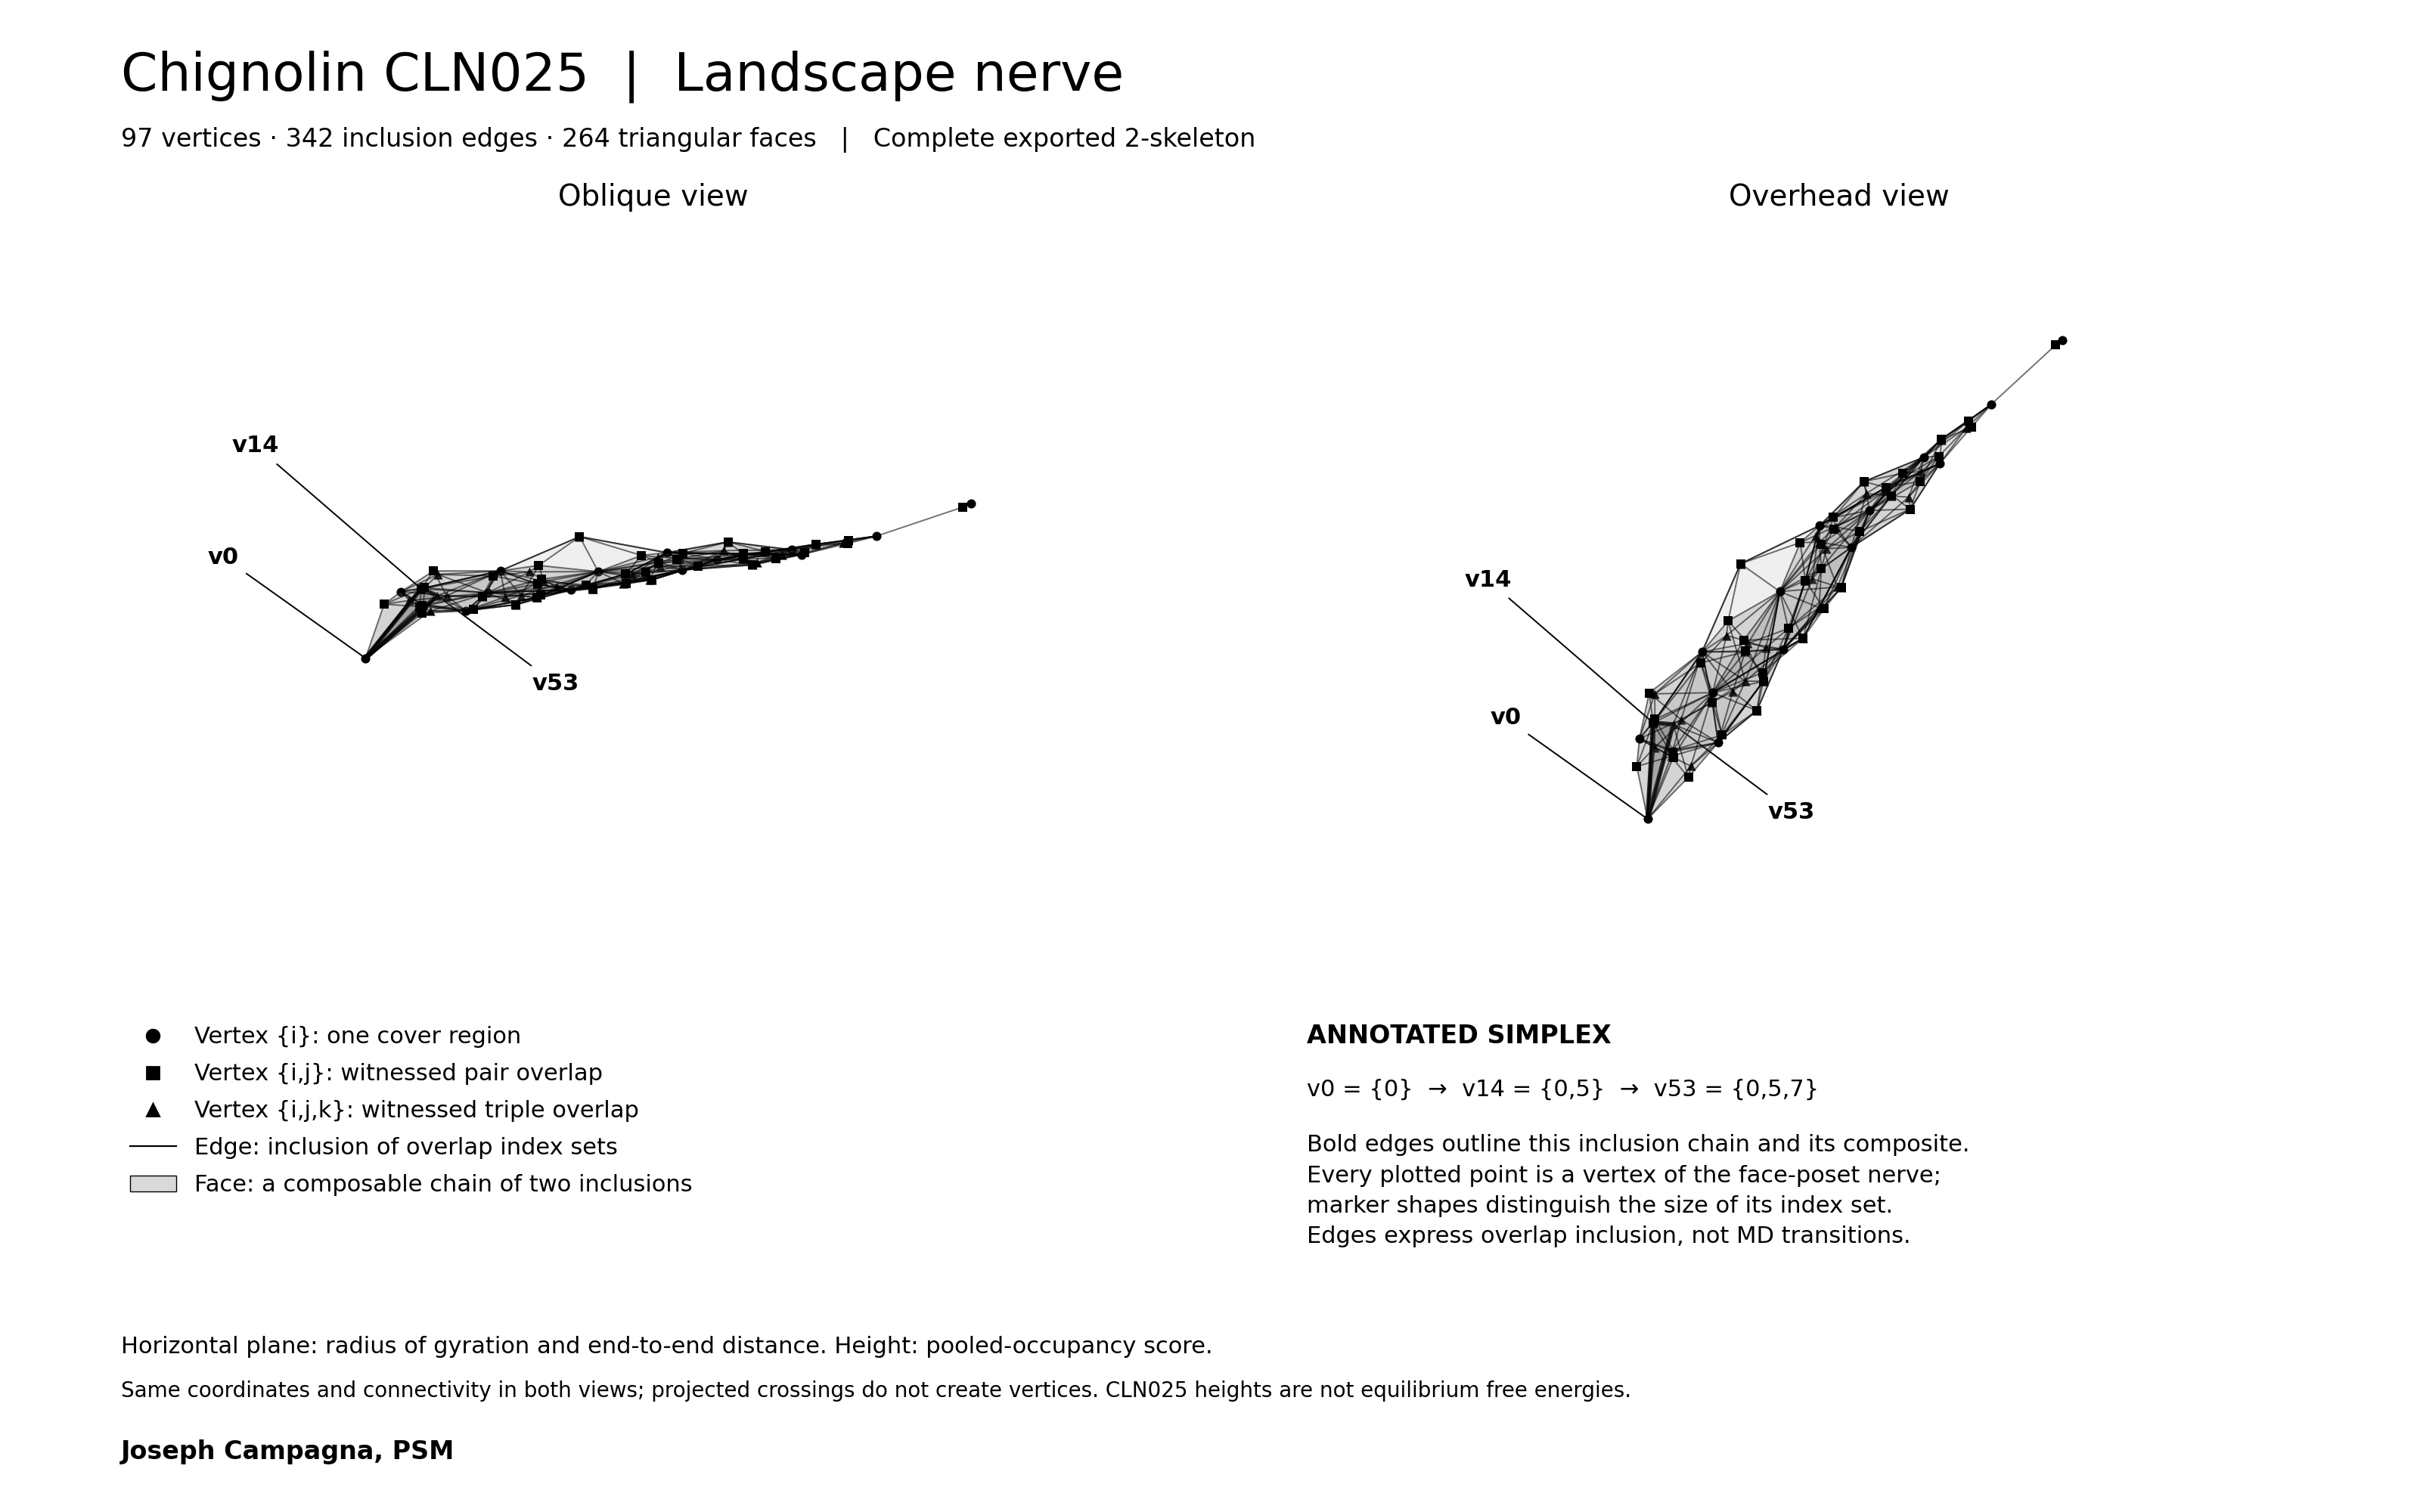
\includegraphics[width=\linewidth]{figures/chignolin-nerve-annotated-both.png}
\caption{\textbf{CLN025: the full exported overlap nerve in two views.}
All 97 vertices, 342 strict inclusion edges and 264 triangular faces are
displayed. The labeled example is
$v_0=\{0\}\subset v_{14}=\{0,5\}\subset v_{53}=\{0,5,7\}$.
The horizontal chart uses C$\alpha$ radius of gyration and end-to-end
distance. Vertical placement follows the viewer's pooled-occupancy score;
it is not an equilibrium free-energy estimate. Marker and edge conventions
match the alanine plate.}
\end{figure}
The elongated geometry reflects the chosen observables and sampled
conformations. It does not establish a folding reaction coordinate or a
topological equivalence with configuration space. The displayed edges are
overlap inclusions, not kinetic pathways; the free path-category overlay
remains a separate construction.

\textbf{Reproducing the plates.}
Run \texttt{python paper/render\_annotated\_nerve.py} from
\texttt{alanine-nerve/}. The script reads the exported node positions,
inclusion edges and chains directly, writes the paired plates into
\texttt{paper/figures/}, and also exports individual viewpoints and SVG
versions into the repository's \texttt{output/nerve-diagrams/annotated/}
directory. No connectivity is inferred from the rendered image.


\newpage
\section*{2. Historical passage construction and revised validation}
The following passage counts describe the original illustrative construction.
They are not promoted to validated kinetics by the new measurement viewer.
The MDshare benchmark contains three independent 250 ns trajectories at
300 K, with 1 ps frame spacing, generated using ACEMD, AMBER ff99SB-ILDN,
and TIP3P water \cite{mdshare}. We use the supplied angles and aligned
heavy-atom positions. All 750,000 frames contribute to occupancy estimates.
Equal-area $12^\circ$ angular bins are smoothed periodically with a Gaussian
of width 0.85 bins:
\[
\widehat E_{\rm occ}(q)=-\log\frac{\widehat p(q)}{\max_{q'}\widehat p(q')}.
\]
Pooling is unweighted. This is an empirical occupancy landscape; equilibrium
convergence and estimator uncertainty have not been established.

Density modes are found separately on a $60\times60$ grid, smoothed at 1.4 bins.
Disjoint $25^\circ$ cores around four peaks define passage labels.
The label $\ell_t$ retains the last core visited between core entries.
Fifteen initial frames, before any core visit, are excluded from labeled counts.

\begin{center}
\begin{tabular}{lrrr}
\toprule Basin & $\phi$ & $\psi$ & Last-core occupancy\\\midrule
A & $-75^\circ$ & $153^\circ$ & 39.57\%\\
B & $-141^\circ$ & $159^\circ$ & 25.62\%\\
C & $-75^\circ$ & $-15^\circ$ & 31.82\%\\
D & $51^\circ$ & $33^\circ$ & 2.99\%\\\bottomrule
\end{tabular}
\end{center}
These are density basins, not demonstrated metastable macrostates.
In particular, A and B interconvert rapidly.
Across independent runs, 73,145 core-to-core passages produce ten directed
route types. Representative counts are A$\to$B: 34,316;
B$\to$A: 34,323; A$\to$C: 1,176; B$\to$D: 1; and D$\to$C: 2.
Sparse directions remain visible and explicitly flagged.

\textbf{Lagged probabilities.}
For lag $\tau\in\{10,50,100\}$ ps, count sliding pairs within each run:
\[
 C_{ij}(\tau)=\sum_r\sum_{t\in I_r(\tau)}
 {\bf1}\{\ell_t^{(r)}=i,\ell_{t+\tau}^{(r)}=j\},
 \qquad
 \widehat P_{ij}(\tau)=\frac{C_{ij}(\tau)}{\sum_k C_{ik}(\tau)}.
\]
Here $I_r(\tau)$ includes only valid labeled pairs in run $r$.
Self transitions are included; pairs never cross run boundaries.
Lagged probabilities may include indirect routes. Sliding observations
are correlated, so row counts are not independent sample sizes.
Gross passage frequency $n_{ij}/750\,\mathrm{ns}$ is distinct from net current.

\textbf{What has been checked.}
Independent counts obtained by removing non-core observations and counting
changes reproduce the passage counts. Exported atomic frames match the raw
coordinates after centering. The first 100 raw coordinate frames reproduce
the supplied torsions to about $2.4\times10^{-7}$ radians.
Probability rows normalize; periodic-distance invariance, endpoint
recovery and within-run lag accounting pass automated checks.

\textbf{Revised validation.}
Implied-timescale, held-out Chapman--Kolmogorov, resampling and stationary-flux
diagnostics are now implemented; the revised CLN025 partitions are fitted
on training groups only. These diagnostics do not establish validated kinetics.
The atlas should not be used to infer new rates, barriers or causal mechanisms.
Section 5 gives the evidence, failed assumptions and outstanding requirements.

\newpage
\section*{3. Chignolin CLN025: extending the atlas}
The second case uses the CC BY 4.0 \emph{Chignolin Simulations} deposit
\cite{chignolin}. Its full dataset comprises 3,744 adaptive-sampling
trajectories of nominal duration 50 ns (187.2 $\mu$s aggregate), generated
with ACEMD, CHARMM22*, TIP3P water and a 350 K Langevin thermostat.
For a bounded, reproducible prototype, we select the first 128 non-hidden
XTC files in archive order. These contain 63,999 frames: 127 runs have
500 frames and one has 499. The selected nominal aggregate duration is
6.4 $\mu$s; it is neither a continuous trajectory nor an unbiased ensemble.

\textbf{Coordinates and chart.}
Ten C$\alpha$ positions are converted from \AA\ to nm, centered, and rigidly
aligned to the first recorded frame by a proper Kabsch rotation.
Neighboring C$\alpha$ distances are checked to lie in $(0.3,0.5)$ nm.
Define geometric, equal-site-weight observables
\[
 R_g(X)=\sqrt{\frac1{10}\sum_{a=1}^{10}\|X_a-\bar X\|^2},
 \qquad d_{\rm ee}(X)=\|X_{10}-X_1\|,\qquad
 q(X)=(R_g,d_{\rm ee})\in\R_{\ge0}^2.
\]
These observables do not require alignment, although consistent alignment
is needed to place molecular shapes in the scene.
The observed coordinate range, padded by 0.01 nm, is mapped linearly to a
$30\times30$ visual chart. A $30\times30$ histogram is Gaussian-smoothed
at 0.85 bins with reflecting boundaries. The displayed score
$E_{\rm occ}(q)=-\log[\widehat p(q)/\widehat p_{\max}]$ is descriptive
negative log occupancy, \emph{not} an equilibrium free energy.

\begin{figure}[H]\centering
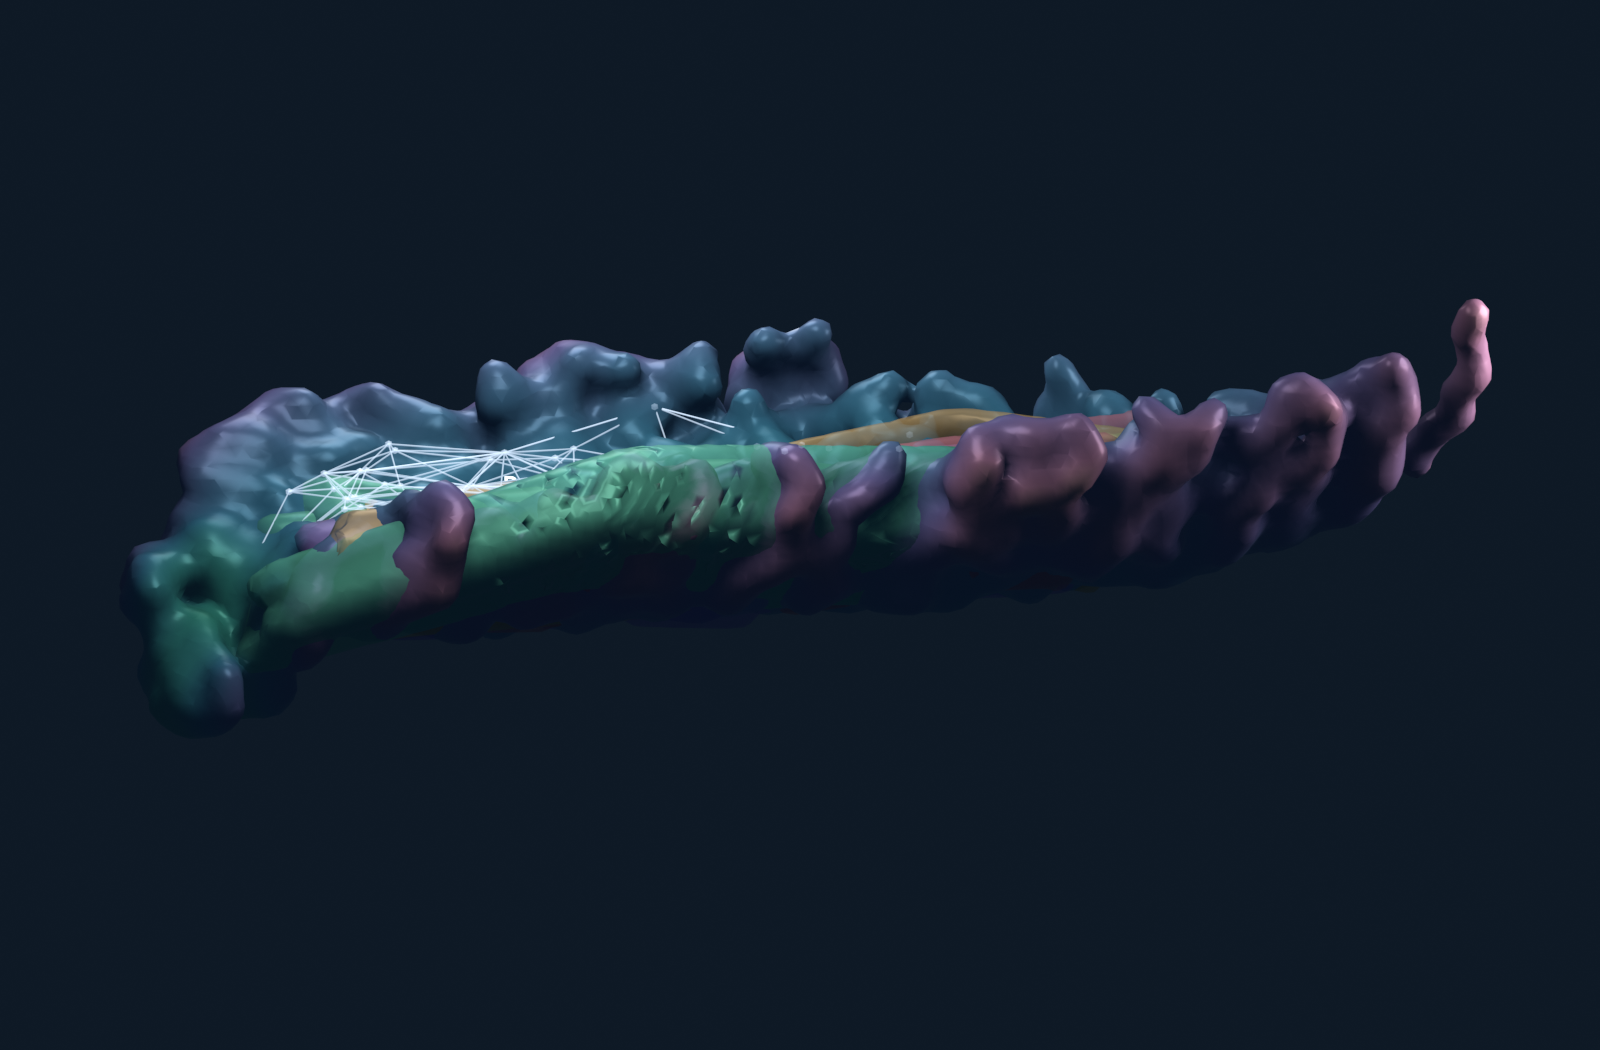
\includegraphics[width=.88\linewidth]{figures/chignolin-landscape-nerve.png}
\caption{\textbf{The CLN025 molecular landscape and overlap nerve.}
Ten-site backbone geometries generate the terrain and deforming pathway
envelopes. Silver lines show inclusions in the overlap face poset.
Horizontal axes encode $R_g$ and $d_{\rm ee}$; height combines
$1.3E_{\rm occ}$ with molecular relief. This is a visualization of the
selected adaptive sample, not a folding free-energy surface.}
\end{figure}

\newpage
\section*{Chignolin transitions and comparison}
Four $k$-means centers are fitted to every fifth observation in standardized
$(R_g,d_{\rm ee})$ coordinates, using seed 42 and 50 iterations.
Centers are ordered by increasing $R_g$ and labeled A--D.
A frame lies in a core when its nearest-center distance is at most 0.42.
The last visited core labels intervening observations. The first 129
pre-core observations are excluded; label memory resets at each run boundary.
There are 6,979 observed core-to-core passages and twelve directed route types.
These clusters are descriptive geometric states, not validated metastable
folding macrostates.

\begin{center}\small
\begin{tabular}{lrr}
\toprule Quantity & Alanine dipeptide & CLN025 subset\\\midrule
Recorded frames & 750,000 & 63,999\\
Independent runs & 3 & 128\\
Temperature & 300 K & 350 K\\
Displayed molecular sites & 10 heavy atoms & 10 C$\alpha$ sites\\
Core-to-core passages & 73,145 & 6,979\\
Observed route types & 10 & 12\\
Overlap nerve objects & 91 & 97\\
Strict inclusion arrows & 282 & 342\\
Overlap 2-simplices & 204 & 264\\
Composable generator pairs & 25 & 36\\\bottomrule
\end{tabular}
\end{center}
Counts compare software constructions, not rates or equivalent dynamical
complexity. Sampling, temperature, molecular resolution and state definitions differ.

\textbf{A finite overlap nerve.}
Fourteen farthest-point centers in the rescaled chart define radius-5.2
Euclidean balls. Every fifth observation witnesses common membership.
As for alanine, the face-poset nerve is formed from the witnessed
2-skeleton. This chart metric is a declared visualization choice;
it is not a physical distance between protein conformations.

\textbf{Pathways and skins.}
Each route uses an actual within-run passage nearest its route's median
duration in frames. At most 80 recorded conformations are retained, and
96 linearly interpolated samples define its envelope. C$\alpha$ coordinates
are magnified by 2.3 visual units/nm; Gaussians have width 0.43, grid spacing
0.30, threshold 0.65, and 0.45-voxel smoothing. The same bounded material
warp as alanine supplies twelve position/normal targets.

\begin{figure}[H]\centering
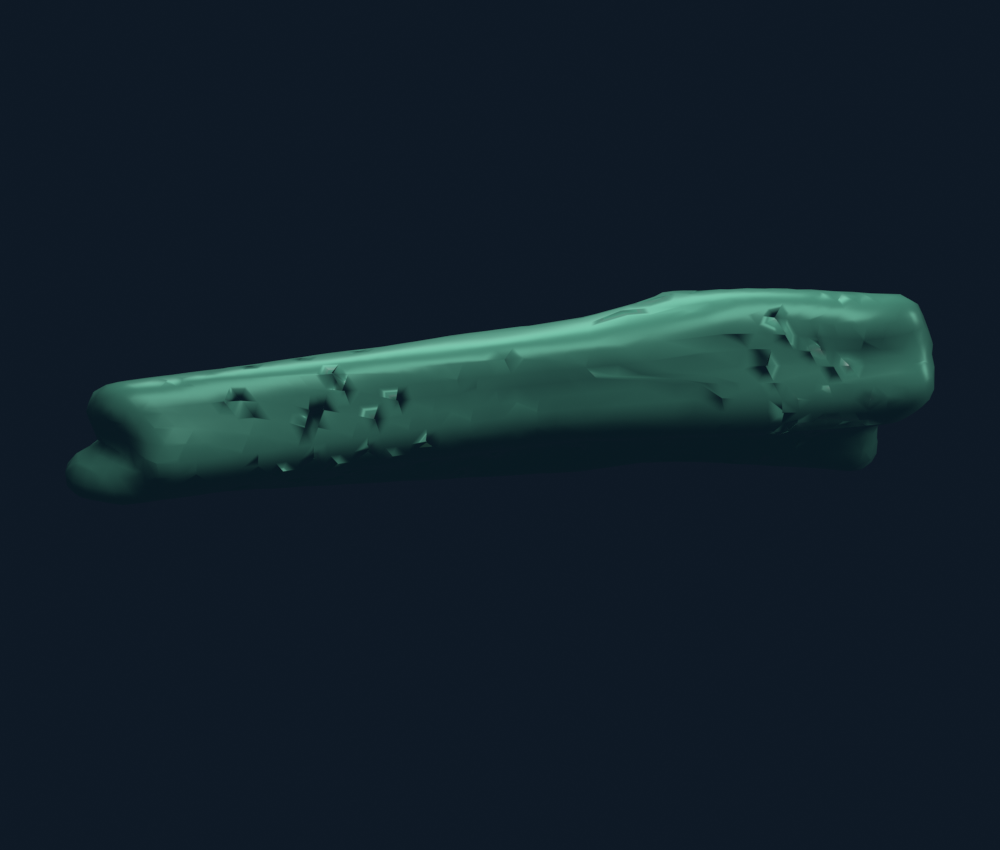
\includegraphics[width=.28\linewidth]{figures/chignolin-phase-0.png}\hfill
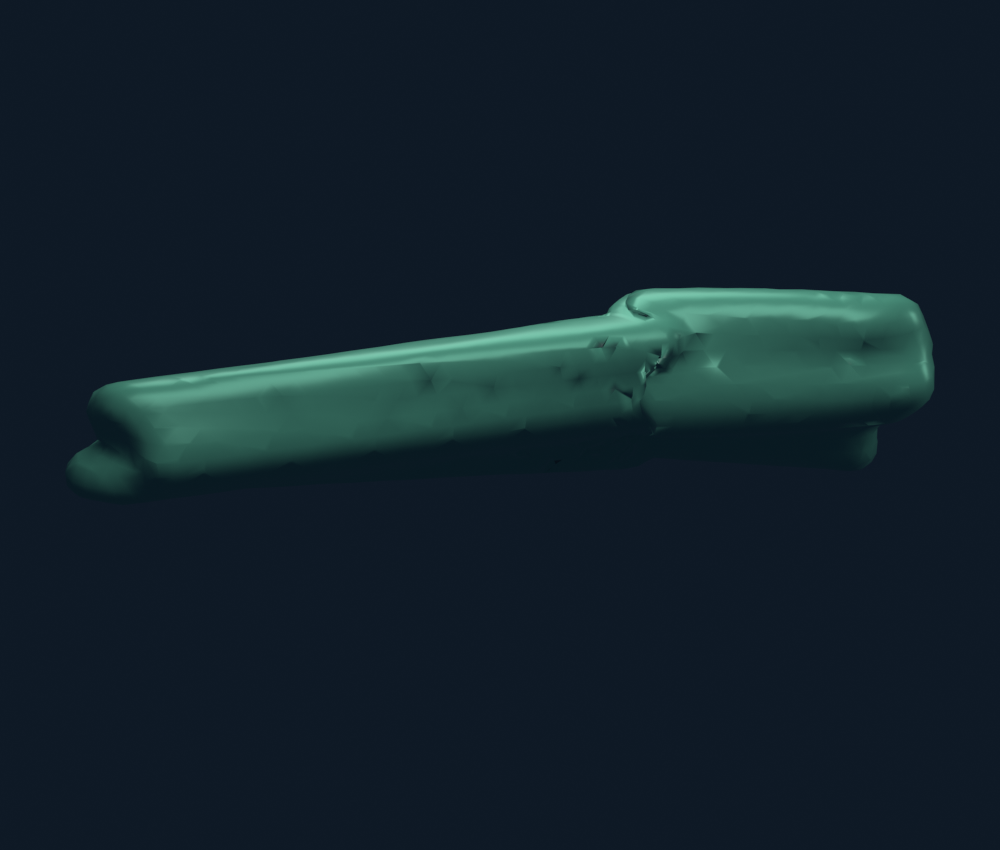
\includegraphics[width=.28\linewidth]{figures/chignolin-phase-1.png}\hfill
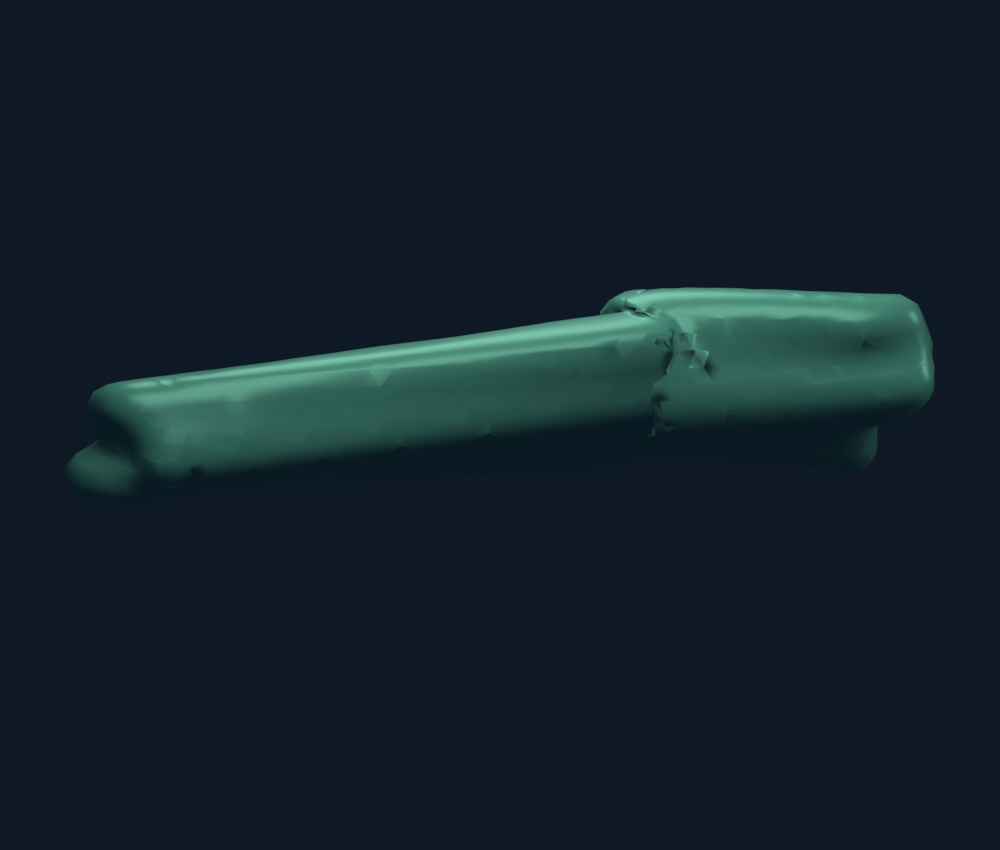
\includegraphics[width=.28\linewidth]{figures/chignolin-phase-2.png}
\caption{\textbf{CLN025 A$\to$C skin at visual phases $0,1/3,2/3$.}
Only this route is shown, under fixed camera and lighting. Surface motion
comes from recorded C$\alpha$ geometry but is not physical time evolution
of a material molecular surface.}
\end{figure}

\newpage
\section*{4. Measured landscapes and the status of continuous skins}
The revised quantitative surface is the supported structural-mobility field
defined in Section 5. Alanine uses a pair-weighted mean; CLN025 uses an equal
mean of root-conditional means with cohort resampling. These are different
descriptive estimands, not comparable free-energy estimates. Molecular relief
uses recorded coordinates under rigid alignment. Playback inserts no synthetic
conformers. Figure 9 replaces the earlier illustrative deformation triptych.

\textbf{Historical skin construction, retained for reproducibility.}
For a representative passage, let $u\in[0,1]$ parameterize its recorded time.
Coordinates are centered and scaled by 3.5 visual units per nm, and translated
to $(\phi/12,\ 1.3\widehat E_{\rm occ},\ \psi/12)$ in the legacy viewer.
Interpolated atomic Gaussians of width 0.36 visual units form a swept envelope:
\[
 \rho_u(x)=\sum_a \exp\!\left[-\frac{\|x-Y_a(u)\|^2}{2(0.36)^2}\right],
 \qquad S=\{x:\max_u\rho_u(x)=0.7\}.
\]
The implementation uses at least 96 temporal samples, a 0.22-unit grid, and
0.45-voxel smoothing before isosurface extraction. Skins share the terrain's
height and molecular scale; they are translucent intersecting meshes, not
a remeshed Boolean union. Cut-chart crossings are not bridged.

\textbf{Actual vertex motion.}
Each skin vertex $v$ receives an approximate nearest-atom phase $u_v$ and
normalized atom weights $w_{va}\propto
\exp[-\|v-Y_a(u_v)\|^2/(2(0.7)^2)]$.
We introduce a bounded material time warp:
\[
 \tau_t(u)=u+0.08\sin(2\pi(t-u))\sin(\pi u),\qquad
 D_v(t)=\sum_a w_{va}\big[Y_a(\tau_t(u_v))-Y_a(u_v)\big].
\]
It fixes the passage endpoints and remains within $[0,1]$.
After two adjacency-averaging steps $L$, the rendered vertex is
\[
 v(t)=v+B_{1.5}\!\left(L^2D_v(t)\right),\qquad
 B_c(z)=c\tanh(\|z\|/c)\frac{z}{\|z\|},\quad B_c(0)=0.
\]
Endpoint-attached displacements are reset to zero. Twelve cyclic keyframes
store both positions and recomputed normals; the browser interpolates between
neighboring targets. A deformation-amplitude control scales the displacement
down to zero for direct comparison with the fixed-envelope version.

\begin{figure}[H]\centering
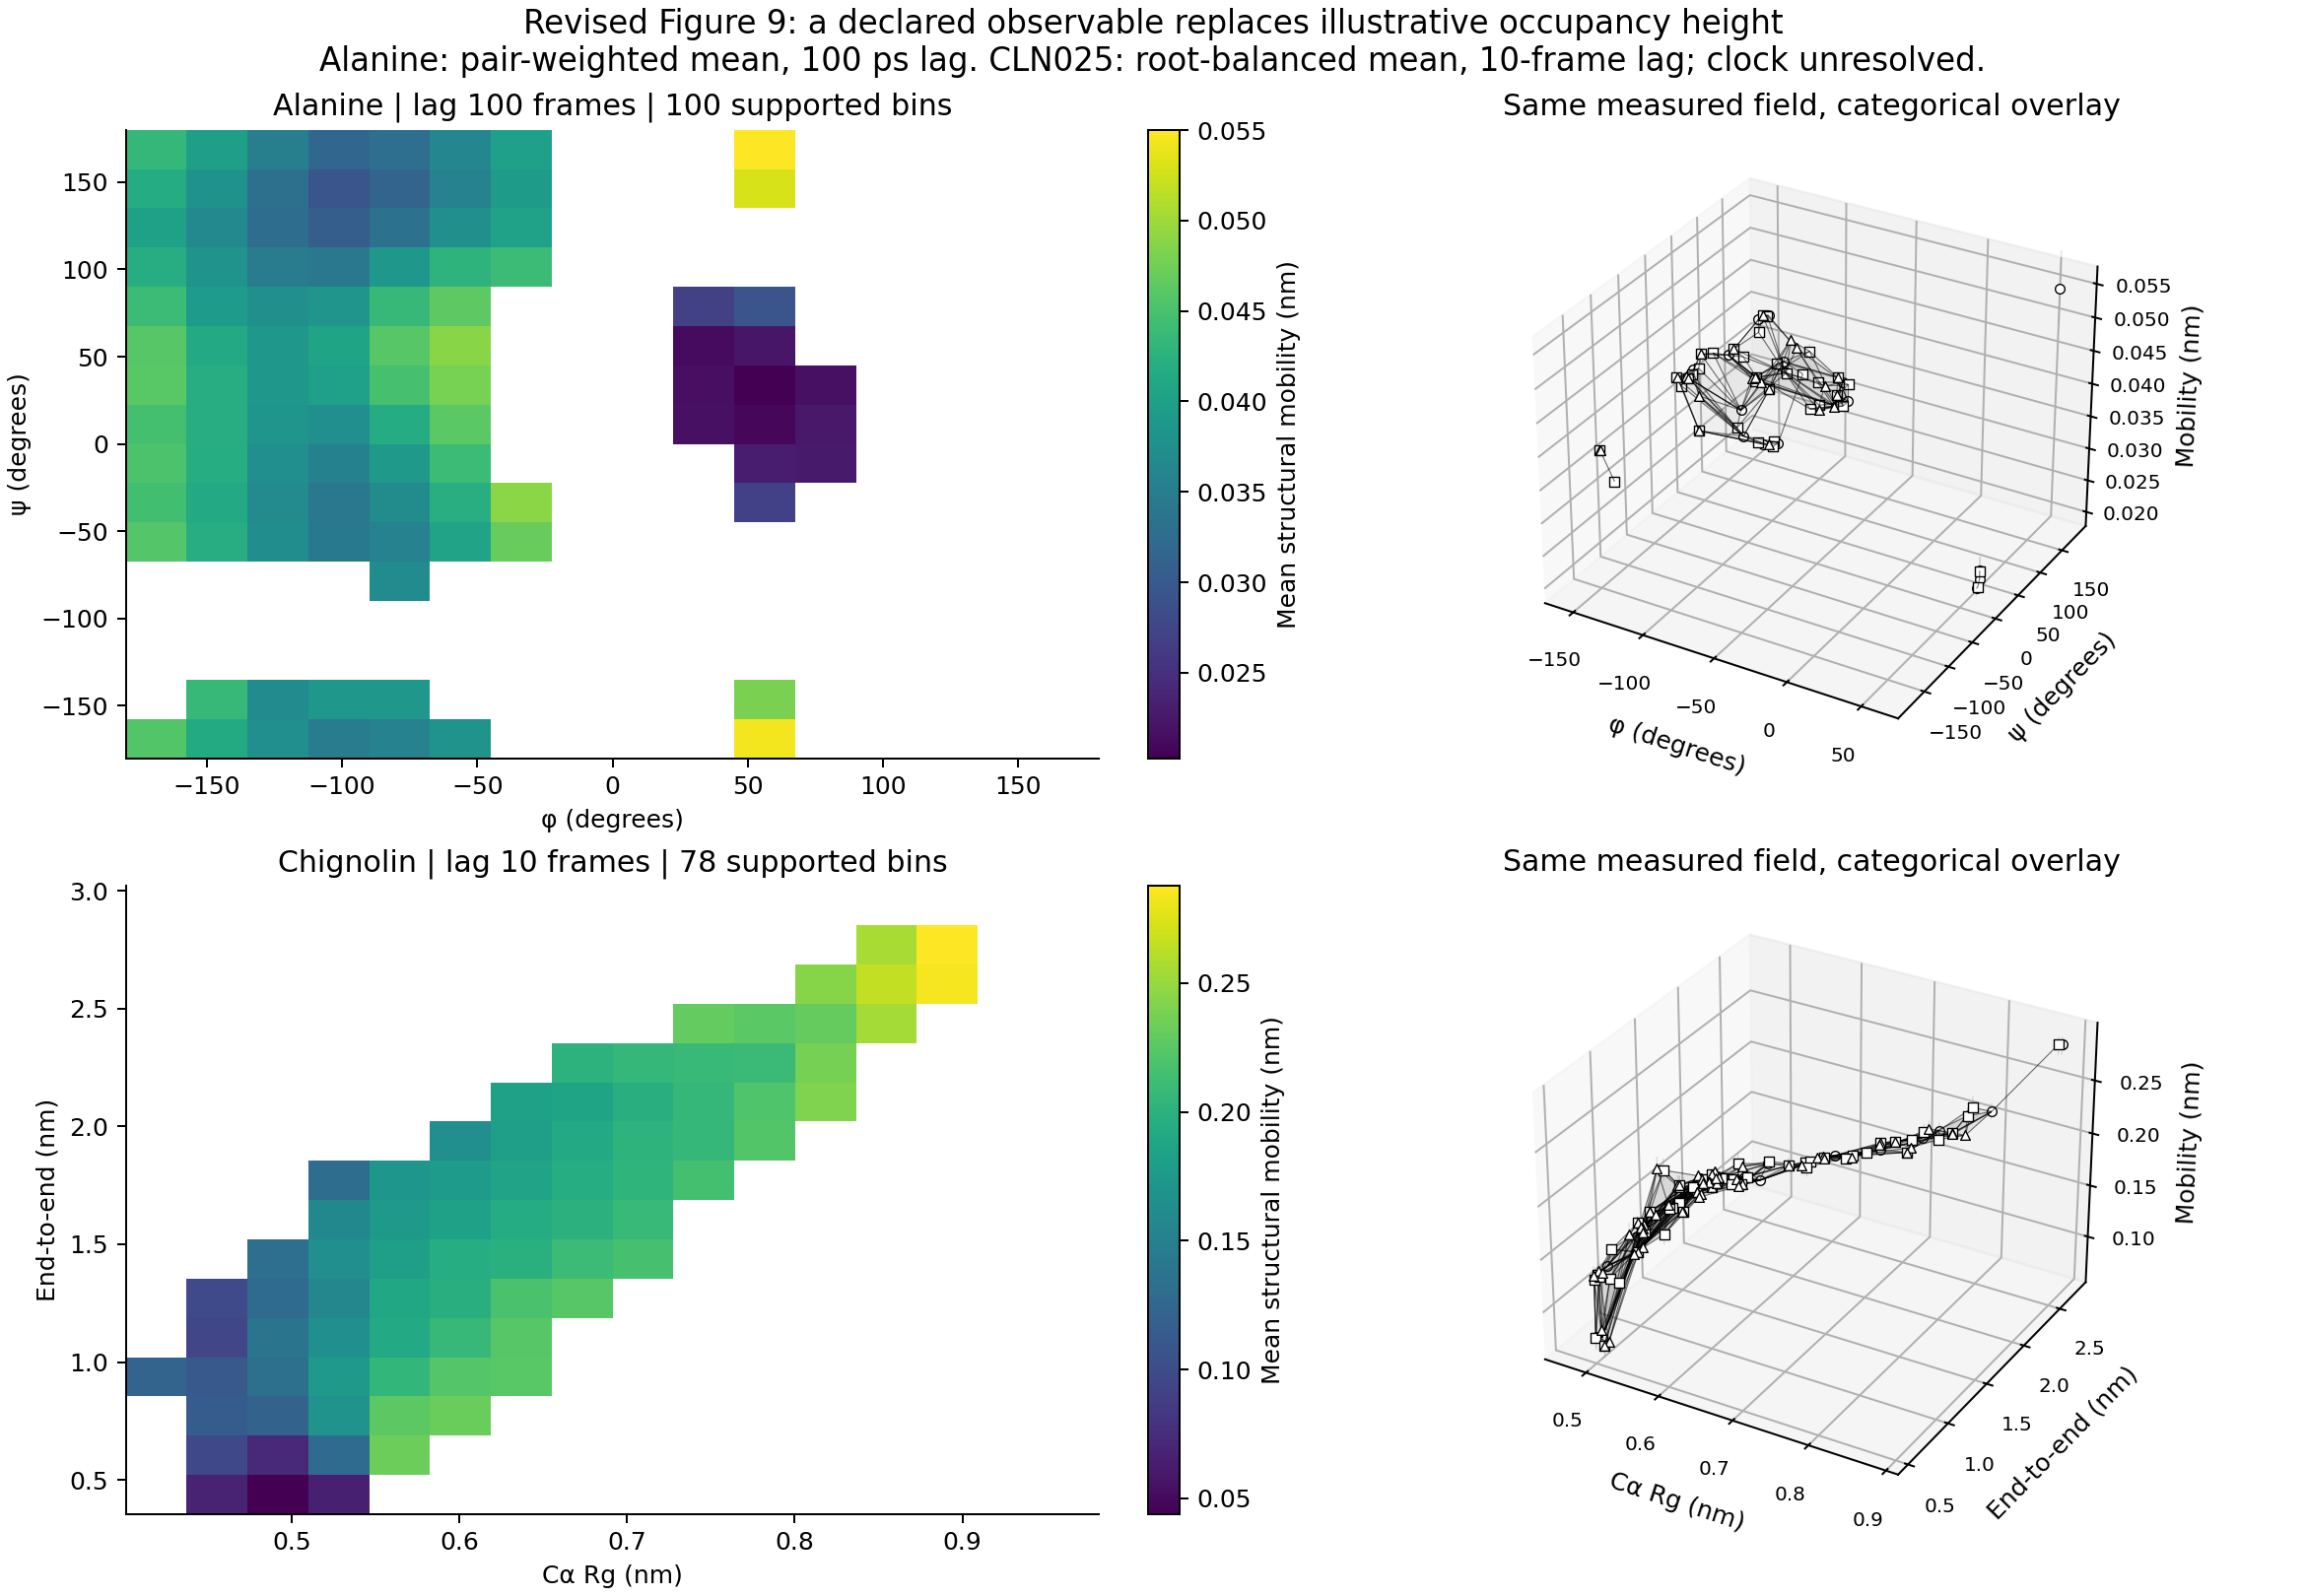
\includegraphics[width=\linewidth]{figures/measured-height-revision.png}
\caption{\textbf{A measured observable replaces illustrative occupancy height.}
Left: supported mean structural mobility; white regions lack reporting support.
Right: the same field supplies heights to the revised overlap-nerve embedding;
bars indicate conditional resampling spread. Alanine uses ten heavy atoms and
a 100 ps lag; CLN025 uses ten C$\alpha$ sites and a ten-frame lag. Averaging,
site selection and lag differ, so the two scales are not thermodynamically
comparable. Heights are in nm, not energy. The flat alanine view omits
seam-crossing geometry; the interactive torus view retains periodic identification.}
\end{figure}
The historical warp is an artistic, MD-attached deformation field. Interpolated Cartesian
coordinates need not preserve bond lengths; self-overlaps can have ambiguous
phase assignments. We do not assert injectivity, volume conservation,
topology preservation, physical forces, or a dynamical semigroup for this animation.

% This file remains an input of paper.tex and also compiles in the open editor.
\ifdefined\AtlasMain
  \let\AtlasSectionEnd\relax
\else
  \documentclass[11pt]{article}
  \usepackage[margin=0.85in]{geometry}
  \usepackage{amsmath,amssymb,booktabs,hyperref}
  \usepackage[T1]{fontenc}
  \usepackage{lmodern}
  \setlength{\parindent}{0pt}
  \setlength{\parskip}{6pt}
  \setlength{\emergencystretch}{2em}
  \hypersetup{colorlinks=true,urlcolor=blue,pdftitle={Molecular Atlas: Revised Limitations},pdfauthor={Joseph Campagna, PSM}}
  \def\AtlasSectionEnd{\end{document}}
  \begin{document}
  {\large\bfseries Molecular Atlas: evidence and remaining limitations}\par
  Joseph Campagna, PSM\hfill Revised October 21, 2026
\fi

\section*{5. Limitations and obstacles encountered}
This revision treats the original limitations in their original order.
Implemented diagnostics are distinguished from successful validation.
The measurement viewer uses supported structural mobility, recorded conformations
and explicitly scoped categorical constructions. Earlier occupancy sculptures
and continuous morphs remain illustrative baselines, not evidence of
thermodynamic or dynamical validity. Evidence is in \texttt{dist/validation/}.

\textbf{1. Dataset scale and selection --- acquisition resolved; sampling scope remains.}
The complete CLN025 archive was checked against its published size
(1,408,223,063 bytes) and MD5, with a retained SHA-256 manifest.
All 3,744 trajectories, containing 1,868,861 frames, are now analyzed.
Extracted member hashes were rechecked; the archive PSF topology was also
recovered and hashed. Actual run lengths determine valid frame pairs;
calculations never join separate runs. The original 128-run, 63,999-frame
selection is retained only as a labeled legacy baseline.
Complete deposit coverage is not complete configuration-space coverage or
statistical representativeness. Evidence: \texttt{01-provenance.json}.

\textbf{2. Timing conflict --- investigated; physical-time claims disabled.}
The XTC interval of 100,000 ps conflicts with the nominal 50 ns production
duration and approximately 500 frames per run. This factor-1,000 discrepancy
persists across the deposit. Archive inventory found topology and frame-count
sidecars, but no production configuration establishing the output stride.
The stated 4 fs integration step does not determine the saved-frame interval.
Raw timestamps are preserved; CLN025 analyses and playback use frame indices,
and the revised export sets its physical frame interval to null.
No physical rate, ns clock, passage time or rate-derived barrier is inferred.
Authoritative output-stride information or corrected files are required;
an inferred rescaling would not resolve the limitation. Alanine retains
its supplied 1 ps frame spacing.

\textbf{3. Adaptive sampling and comparability --- estimands changed; equilibrium unestablished.}
Filename ancestry identifies 100 roots; the largest has 2,505 descendant runs.
Root-directory suffixes identify ten initial-conformation cohorts, consistent
with the deposit's description of ten starting preparations. All descendants
of a cohort stay together in the stronger holdout and resampling analysis.
The four holdout folds contain 2,562, 559, 305 and 318 trajectories.
These conservative filename-derived groupings are not verified restart logs
or certificates of independence.

No pooled CLN025 mobility bin meets the revised threshold of three effective
cohort contributions. That failed-support result is retained. The displayed
CLN025 height is therefore a \emph{different descriptive estimand}: an equal
average of root-conditional means. For chart bin $B$,
\[
 m_\ell(t)=\left[\frac{1}{45}\sum_{a<b}
 \big(d_{ab}(X_{t+\ell})-d_{ab}(X_t)\big)^2\right]^{1/2},
 \qquad
 h_B=\frac{1}{|\mathcal R_B|}\sum_{r\in\mathcal R_B}\overline m_{r,B}.
\]
Roots in $\mathcal R_B$ must have at least 20 retained within-run lag pairs
in $B$. Entire initial-conformation cohorts are resampled together.
Equal root averaging is not Boltzmann weighting or an equilibrium correction;
the contributing-root mixture can vary between bins. Alanine instead uses
a pair-weighted conditional mean and within-run block resampling.
Lags are 100 ps for alanine and ten frames for CLN025. Different sites, lags,
temperatures, force fields and averaging conventions prevent thermodynamic
comparison of the two height scales.

Support requires 100 retained pairs, five blocks, three runs, three resampling
units and three effective unit contributions. The last diagnostic is
$(\sum_c w_c)^2/\sum_c w_c^2$; it is not an effective sample size corrected
for all temporal dependence. The fields retain 100 alanine bins and 78 CLN025
bins. Missing support is not filled or assigned zero. Lag, block-length and
bin-resolution sensitivities are exported. Percentile intervals remain
conditional resampling spread, not calibrated confidence intervals.
Evidence: the atlas, pooled-height and initial-cohort JSON files, and
\texttt{06-topology-height-sensitivity.json}.

\textbf{4. Chemical identity and cartoons --- mapping and geometry checks strengthened.}
The dataset is capped CLN025, YYDPETGTWY, not original chignolin.
The recovered PSF contains 177 atoms and 180 bonds: 175 peptide/cap atoms
and two sodium ions. PSF and PDB atom names agree. CAY/CY/OY and NT/CAT
identify the deposited acetyl and methylamide caps. The PSF stores nominal
masses, whereas the deposit describes hydrogen mass repartitioning; it does
not establish the integrator's actual masses.

Every CLN025 frame was screened using PSF heavy-atom bonds and orthorhombic
minimum-image reconstruction of the ordered backbone. No backbone reconstruction
changed a frame. Heavy-bond distances ranged from 0.10889 to 0.17719 nm;
none failed the broad 0.10--0.20 nm anomaly screen. This is not an energy
or steric-clash certificate. All peptide omega angles were extracted:
66 observations have cis Asp3--Pro4 geometry and are retained. The old universal
0.3 nm minimum C$\alpha$ spacing is withdrawn as a validity criterion.
All 750,000 alanine coordinate frames reproduce the supplied torsions within
$3.49\times10^{-7}$ radians and pass the broad bond screen. Its supplied
aligned coordinates lack per-frame periodic cells; those cells are not invented.

The 20-member \href{https://www.rcsb.org/structure/2RVD}{2RVD NMR ensemble}
supplies an explicit sequence-matched structural reference. Minimum RMS
discrepancy in nonlocal C$\alpha$ pair distances is a continuous similarity
observable, not a native-state assignment. Caps and experimental conditions
differ. No folding threshold, hydrogen-bond network or secondary structure
is inferred from a smooth cartoon. Recorded sites and straight connection
guides are available without Cartesian interpolation.
Evidence: \texttt{04-chemistry.json}, \texttt{04-alanine-chemistry.json}
and recorded-conformation exports.

\textbf{5. Projection and state definitions --- alternatives tested; no preferred interface declared.}
The $(R_g,d_{\rm ee})$ chart remains a visualization coordinate system,
not a sufficient dynamical state. Nested grouped validation compares the chart,
45 C$\alpha$ distances, periodic phi/psi/omega features, their combination,
and a combination with 20-frame history. Future targets are distances,
periodic omega and NMR-distance deviation at ten- and 50-frame lags.
Scaling and ridge-parameter selection use training groups only; persistence
is the baseline. Both root and initial-cohort holdouts are retained.
This reduces the earlier bias from evaluating distance inputs against only
a distance target, but does not exhaust nonlinear models, memory or solvent
variables. Partitions with 4, 8 and 16 clusters are separately fitted on
training data for kinetic checks. No best torsion/contact interface,
metastability, reaction coordinate or Markov closure is inferred.
Evidence: \texttt{05-predictive-validation*.json}.

\textbf{6. Categorical claims --- finite constructions corrected; space-recovery theorem not claimed.}
Both witnessed covers are rebuilt from all available frames. Alanine uses
the periodic angular metric with displayed radius $55^\circ$; CLN025 uses
radius 0.8 in standardized chart coordinates. Maximal simplices retain the
complete finite witnessed complexes, of maximal dimensions three and five.
Tetrahedral boundaries are included in computing $H_2$ over $\mathbb F_2$;
discarding them can manufacture apparent cavities. Cover-scale and
witness-stride sensitivities are retained. Alanine's Betti numbers vary
with radius, so stable configuration-space topology has not been established.

The drawing is the 2-skeleton of $N(P(K_W^{(2)}))$, not every simplex of $K_W$.
It has 78 objects, 212 inclusions and 138 triangular chains for alanine;
CLN025 has 131 objects, 466 inclusions and 360 chains. Two alanine objects
lack supported heights and are omitted only from the embedding. Their
categorical records remain. The interactive torus view respects angular
identifications; the flat cut view omits seam-crossing geometry rather than
joining it by false long chords. Drawing intersections create no new incidences.

For $\sigma\subset\tau$, witness sets satisfy $W_\tau\subset W_\sigma$:
witness inclusion is a contravariant finite-set interpretation, not an
identification with the free path category. Closure, inclusion composition
and simplex preservation have executable tests. Good-cover assumptions,
unseen intersections, projection-induced merging, a comparison functor to
molecular path dynamics and a proof-assistant export remain unestablished.
The exact barycentric-subdivision statement does not establish recovery
of molecular configuration-space homotopy.

\textbf{7. Statistical and dynamical validation --- diagnostics expanded; kinetic claims withheld.}
Training-only partitions are checked at 5-, 10- and 50-frame lags, with
held-out two- and four-step Chapman--Kolmogorov comparisons. Each state row
retains counts, predicted/observed probabilities, total-variation discrepancy
and conditional group-resampling spread. Rows below 100 pairs are flagged;
unsupported rows remain missing, not absorbing. Weighted averages do not
replace worst-row reporting. In initial-cohort holdouts, ten-frame weighted
discrepancies span approximately 0.055--0.270 across tested configurations;
the maximum single-row discrepancy across configurations is approximately
0.460. These results do not establish validated kinetics. Last-core labels
remain explicitly distinguished from instantaneous states.

A known-process experiment illustrates the dependence problem. Across 200
synthetic trials, nominal 95\% percentile intervals covered the known transition
probability in 90\% of trials when ten independent cohorts were resampled,
but only 40.5\% when duplicated descendants were incorrectly treated as
independent roots. This synthetic result neither calibrates MD uncertainty
nor validates molecular dynamics. Independent preparations, experimental
checks, model-selection uncertainty and rare-event coverage remain necessary.

An executable finite-stochastic-kernel contract specifies finite state sets,
identity matrices and row-convention composition $P;Q=PQ$. Identity and
associativity are tested; algebraic composition does not imply
$P_{\rm observed}(2\ell)=P(\ell)^2$. A naive independent-product model of
median-split $R_g$ and end-to-end distance has a ten-frame worst-row discrepancy
near 0.497 against the observed joint kernel. These observables cannot simply
be declared independent compositional modules. Boundary variables, admissible
couplings, behavior semantics and composed-versus-joint predictive agreement
remain research requirements. Evidence: \texttt{07-kinetic-validation*.json},
\texttt{07-synthetic-coverage.json} and \texttt{composition-contract.json}.

\textbf{8. Deformation and geometry --- unsupported interpretation removed; continuous repair incomplete.}
The legacy audit identified disconnected components. The new screen evaluates
48 phases per route, including intermediate positions between stored targets.
All 22 route skins have nonadjacent BVH overlap candidates at some sampled
phase. These are candidates, not an exact continuous-time intersection
certificate; adjacent-face crossings and inter-object collisions are not
exhaustively certified. Bounded displacement does not imply injectivity,
conserved volume, topology preservation, valid bonds or a physical law.
Boolean union would not repair these scientific limitations.

The measurement viewer therefore uses recorded conformers under proper rigid
alignment only. Playback steps through actual frames without synthetic
molecular intermediates. Pair-distance invariance is checked. Measured tile
heights, magnified molecular relief and the lifted nerve have separate visual
roles. Figure 9 is replaced by mobility fields and measured-height nerves.
Continuous glossy skins remain separately labeled artistic assets.
A physical smooth field requires a validated correspondence, chemical
constraints and collision checks throughout interpolation; realistic materials
supply none of these. Evidence: \texttt{08-geometry.json} and recorded exports.

\textbf{9. Rendering and software constraints --- reproducibility and checks strengthened.}
The measurement viewer provides local vendored dependencies, missing-support
masks, recorded-frame controls, separate nerve plates and conditional spread
bars. Quantitative tile colors use unlit materials; molecular relief uses
fixed lighting. Revised Blender figures use measured heights, recorded sites
and geometric normals, with optical appearance separate from the numerical field.
Scientific dependencies are pinned for the tested Python environment;
browser-test dependencies have a package lock. Tests cover run boundaries,
missing rows, rigid invariance, periodic distance, higher simplices, cohort
grouping, root-balanced averaging and stochastic composition.
Headless Chrome and Edge checks exercise both systems, playback, torus view,
layer controls and mobile layout, followed by screenshot review.
Both use Chromium and the available NVIDIA stack; this is not cross-engine
or universal hardware certification. MDAnalysis remains the working parser;
no unused MDTraj dependency is introduced. HTTP serving remains required.
Evidence: \texttt{09-browser-checks.json}, tests, environment record and locks.

\textbf{10. Publication and reproducibility scope --- coherent local revision; publication separate.}
Ordered remediation scripts, compact validation data and revised figure/manuscript
sources accompany the preserved illustrative baseline. Raw trajectories remain
separately downloadable and attributed; source/output hashes provide traceability.
No new GitHub publication, workflow authorization, external message or Instagram
upload is implied by local validation. The existing public viewer and previously
published PDF remain historical until a coordinated release.
This pass updates the open limitations source and its compiler preview; it
does not silently replace the published manuscript PDF. Older Git history
can still contain previously tracked artifacts. A release should version source,
manifests, figures and the complete manuscript together.
The work remains exploratory and not peer reviewed.

\subsection*{Remaining acceptance gates and future directions}
Recover authoritative CLN025 timing and restart provenance first.
Test uncertainty and predictive closure with independent preparations,
rare states and experimental observables. Validate equilibrium estimation
before introducing $-k_BT\log\pi$ as a height; committor and passage-time
heights additionally require justified boundary sets and kinetics.
Refine cover/projection sensitivity before any configuration-space theorem.
For smooth surfaces, validate $\Phi_\theta$ and its tangent map before
interpreting $(D\Phi_\theta)^{\mathsf T}D\Phi_\theta$ as a molecular
deformation metric. Then select and test interfaces and coupling laws for
composed dynamics. Synthetic differential geometry is an optional framework
for smooth infinitesimal semantics, not a substitute for these prerequisites.

\AtlasSectionEnd

\newpage
\section*{6. Future directions}
The current construction makes \emph{path composition} inspectable.
Composing complete dynamical subsystems is a stronger objective.
For an autonomous flow, one expects
$\Phi_{t+s}=\Phi_t\circ\Phi_s$; a Markov approximation would analogously
require $P(t+s)\approx P(t)P(s)$ under a stated convention.
Neither property follows from drawing a nerve.

One proposed next step is to define structural interfaces (for example,
selected contact or torsional observables), attach validated dynamics to
modules, and specify how compatible interfaces compose.
Open reaction networks and open Markov processes provide established
categorical examples: input/output boundaries allow systems to compose,
and functorial semantics can relate composite models to their behavior
\cite{baez,pollard}. Applying such ideas to structural bioinformatics would
require new choices and validation, not just a change in visualization.

The research questions are concrete:
\begin{enumerate}
\item Can basin definitions and transition estimates remain stable across
trajectory blocks, temperatures, and resolutions?
\item Can experimentally meaningful interfaces support compositional
models with quantified approximation error?
\item Can a semantics functor $\mathcal S:\mathcal D\to\mathcal B$ satisfy
$\mathcal S(g\circ f)=\mathcal S(g)\circ\mathcal S(f)$, where $\mathcal D$
is a category of specified open models and $\mathcal B$ their behaviors?
\item Extend the completed distance/phi/psi/omega/history comparisons with
native-contact and hydrogen-bond observables, nonlinear predictive models
and experimentally interpretable targets. The NMR-distance reference is
not yet a native-state definition or a folding validation.
\item Resolve the timestamp discrepancy and verify restart/cohort provenance.
The full archive and grouped kinetic diagnostics are now analyzed; the
remaining tasks are justified equilibrium estimation, calibrated uncertainty
and genuinely independent predictive checks, not merely more pooled frames.
\item Can an explicitly defined projection between atomistic and C$\alpha$
state categories preserve specified compositions? Such a comparison functor,
including its approximation error, would connect the two visualization scales.
\end{enumerate}
Here $\mathcal D$, $\mathcal B$, and $\mathcal S$ are research targets,
not artifacts implemented by this prototype.
Homotopy.io offers a useful reference for higher-categorical diagramming
\cite{homotopy}; the current viewer is a custom Three.js implementation,
without a homotopy.io export or proof certificate.

\textbf{Reproducibility.}
The companion source includes data-download and analysis scripts,
MD-driven morph targets, the LaTeX source, a Blender scene with shape keys,
and the figure-generation script. The browser and Blender use the same
geometry. The underlying source-file SHA-256 hashes are recorded in
\texttt{dist/data.json}. Regenerate in this order:
\texttt{download.py}, \texttt{prepare.py}, \texttt{dynamics.py},
\texttt{build\_skins.py}, \texttt{build\_deformation.py}.
For CLN025, run \texttt{download\_chignolin.py} then \texttt{build\_chignolin.py}.
The repository provides a static viewer, runnable tests and both figure pipelines.
The figures use Blender 4.0/Eevee; the document is compiled from LaTeX.

\textbf{Exploratory proposition.}
Categorical language may help separate state, transition, composition,
and interface in molecular modeling. This atlas offers a visible,
inspectable starting point for that discussion, rather than evidence
that categorification has already improved a predictive model.

\newpage
\section*{7. Availability, attribution and references}
\textbf{Software and paper.}
\url{https://github.com/joecampdb/pronerv_MTNerv}.
The molecular atlas lives in \texttt{alanine-nerve/}; its historical directory
name is retained for compatibility. The repository also retains an independent
polyethylene screening workflow, documented separately. The compiled paper is
\texttt{paper/molecular-atlas.pdf} at repository root.

\textbf{Data and transformations.}
The CLN025 data are attributed to Adri\`a P\'erez Culubret and Gianni De Fabritiis
under CC BY 4.0 \cite{chignolin}. The subset is streamed in archive order;
individual PDB/XTC SHA-256 hashes and exact member names are retained.
Transformations include C$\alpha$ selection, centering, rigid alignment, geometric
features, clustering, density estimation, subsampling, and visual surface extraction.
The original archive is approximately 1.41 GB; only the selected members are read.
The deposit's archive MD5 is recorded as metadata, not asserted to have been
verified against a complete local download.

\textbf{Interpretation of the two examples.}
Alanine is a torsional benchmark; CLN025 is a ten-residue mini-protein variant.
The extension demonstrates that the software can represent a more complicated
conformational dataset, not that the same two-dimensional representation
resolves its folding kinetics. No quantitative performance gain from
categorification has been established.

\textbf{Authorship and preparation.} Joseph Campagna, PSM.
This exploratory software and manuscript were prepared with AI-assisted coding
and drafting. Numerical outputs and figure sources are included for inspection;
the document has not undergone peer review.

\footnotesize
\begin{thebibliography}{9}\setlength{\itemsep}{1pt}
\bibitem{mdshare} MDshare. \emph{Alanine dipeptide dataset and simulation metadata}.
\url{https://markovmodel.github.io/mdshare/ALA2/}.
\bibitem{may} J. P. May. \emph{Simplicial sets, nerves of categories, Kan complexes, etc.}
\url{https://math.uchicago.edu/~may/REU2018/sset.pdf}.
\bibitem{bauer} U. Bauer, M. Kerber, F. Roll, A. Rolle.
\emph{A Unified View on the Functorial Nerve Theorem and its Variations}.
\url{https://arxiv.org/abs/2203.03571}.
\bibitem{baez} J. C. Baez, B. S. Pollard.
\emph{A Compositional Framework for Reaction Networks} (2017).
\url{https://arxiv.org/abs/1704.02051}.
\bibitem{pollard} B. S. Pollard. \emph{Open Markov Processes and Reaction Networks} (2017).
\url{https://arxiv.org/abs/1709.09743}.
\bibitem{homotopy} N. Corbyn et al.
\emph{homotopy.io: a proof assistant for finitely-presented globular $n$-categories} (2024).
\url{https://arxiv.org/abs/2402.13179}.
\bibitem{chignolin} A. P\'erez Culubret and G. De Fabritiis.
\emph{Chignolin Simulations} (2021), Figshare, CC BY 4.0.
\url{https://doi.org/10.6084/m9.figshare.13858898}.
\end{thebibliography}
\end{document}
